\chapter{Hardware di destinazione}
    
Come è stato scritto nell'introduzione la scheda \textit{Arduino Uno R3} è stata scelta per velocizzare lo sviluppo e per permettere al progetto di essere accessibile per un considerevole numero di utenti tenendo in considerazione le capacità e le competenze del segmento di pubblico al quale la scheda è rivolta.

\begin{figure}[b]
    \centering
    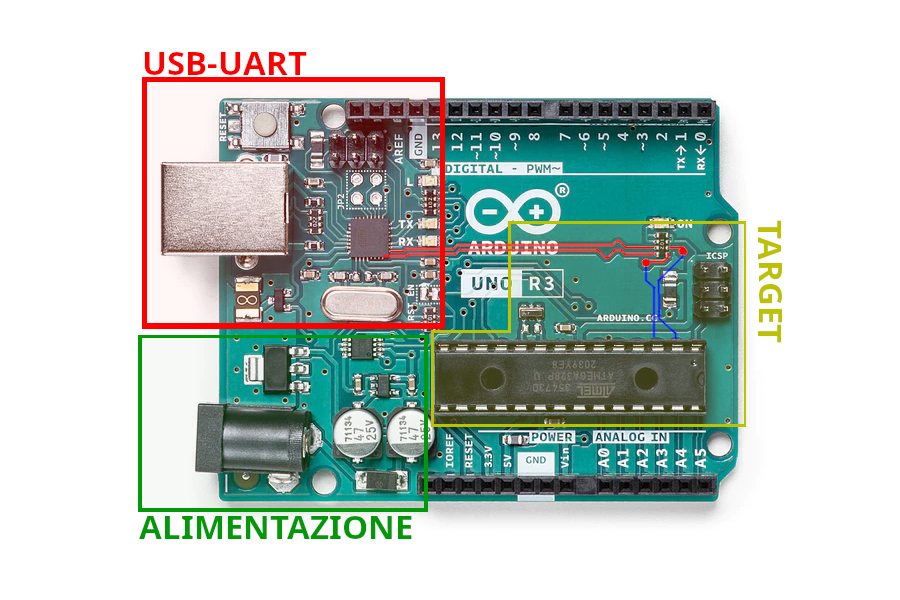
\includegraphics[width=.5\textwidth]{arduino-uno.png}
    \caption[]{Foto di una scheda Arduino Uno R3\cite{img:arduino-uno-r3}}\label{fig:arduino-uno-r3}
\end{figure}

la scheda (Figura~\ref{fig:arduino-uno-r3}) presenta una serie di connettori posti ai lati, collegati ai pin del controllore principale in centro, utili per interconnettere il dispositivo con i circuiti in sviluppo.
L'hardware addizionale presente sul lato sinistro --- invece --- permette di alimentare la scheda da una sorgente esterna non regolata tramite il connettore cilindrico nero e di collegare il controllore principale, tramite connessione seriale, a un computer tramite la porta USB presente in alto a sinistra.
È inoltre possibile effettuare il reset manuale del target tramite il pulsante presente vicino alla presa USB.

Il controllore presente al centro della scheda, in un involucro DIP-28\footnote{Dual in-line package, 28 pin}, è un ATMega328P-PU\cite{site:arduino-uno-doc}. È stato scelto un formato così ``datato'' per permettere all'utente di sostituire il chip in caso di guasto.

\section{La famiglia AVR}

Il controllore ATMega328P-PU presente sulla scheda di sviluppo è un membro della famiglia AVR di Atmel\cite{avr:m328p}.

Come è possibile identificare dalla figura~\ref{fig:avr-arch} l'architettura del processore della famiglia AVR è di tipo Harvard: È evidente la dicotomia tra memoria del programma (nell'immagine ``\textit{Flash Program Memory}''), SRAM e EEPROM\cite{harvard-arch}.

La suddivisione consente di ottimizzare separatamente le due diverse tecnologie di storge intrinsecamente diverse.

Come è possibile osservare, la grandezza del bus dati è di 8 bit, di conseguenza è possibile dedurre che l'intera architettura si basa sull'unità fondamentale del byte.

Vi è poi la totale assenza di pipelining essendo un processore a singolo ciclo. La maggior parte delle istruzioni, infatti, viene eseguita in un solo ciclo di clock\cite{avr:m328p} ad esclusione delle operazioni sulle memorie le quali ``stallano'' il processore per questioni di tempi di accesso/scrittura o di istruzioni che involvono dati di lunghezza maggiore di 8 bit.

\begin{figure}[t]
    \centering
    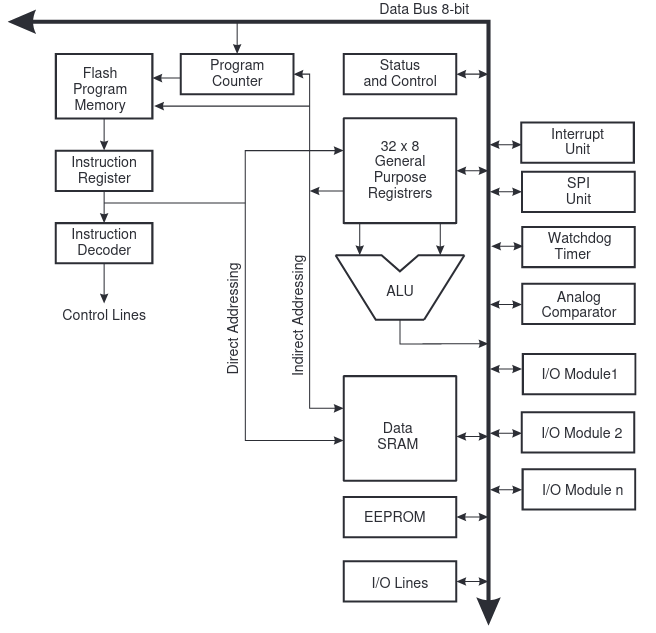
\includegraphics[width=.9\textwidth]{avr_arch.png}
    \caption[]{Schema a blocchi dell'architettura AVR\cite{avr:m328p}}\label{fig:avr-arch}
\end{figure}

\subsection{Memorie}

All'interno di ogni processore AVR sono presenti tre differenti tipi di memorie: Flash, SRAM e EEPROM.

La memoria Flash è generalmente la memoria più capiente del controllore e in genere la sua dimensione contribuisce nella denominazione della parte. È una memoria ad accesso casuale in lettura ma, a differenza di quanto ci si possa attendere, la dimensione dell'unità di dati elementare è di 16 bit.

La dimensione di 16bit per unità è utilizzata in quanto tutte le istruzioni dell'\textit{Instruction Set} hanno dimensione di 16 o 32 bit.\cite{avr:isa}.

La memoria Flash può essere scritta tramite un programmatore esterno (ISP\footnote{In System Programmer}) oppure mediante una procedura di \textit{auto-programmazione} tramite l'istruzione SPM.
La memoria non viene mai utilizzata come uno storage permanente in quanto necessita che la scrittura avvenga per pagine di 512/1024 bit in funzione dell'implementazione. Questo comporta alti tempi di riprogrammazione rendendo così l'utilizzo di questa memoria come storage non volatile inefficiente.

La memoria flash viene indicizzata dal program counter (escludendo il bit meno significativo) e il risultato viene salvato sempre nell'instruction register. 
La mancanza di un collegamento tra Flash e bus dati sembrerebbe implicare l'impossibilità di leggere dati da essa durante l'esecuzione. 
Contrariamente a questa aspettativa, l'operazione viene implementata leggendo il contenuto della flash salvandolo nell'instruction register (I ciclo) e successivamente copiando il contenuto del IR nel registro di destinazione (II ciclo). Nello stesso ciclo viene effettuata la lettura della prossima istruzione e viene aggiornato l'IR. 

La sezione dedicata allo storage non volatile è invece la memoria EEPROM. Quest'ultima consiste in un array di celle dalla dimensione di un byte singolarmente leggibili e scrivibili in tempi contenuti.
L'utilità della EEPROM è subito evidente: grazie a questa memoria è possibile salvare dati che verranno preservati in caso di mancanza di alimentazione; tenendo conto che i controllori AVR presentano una soluzione integrata in grado di permettere allo sviluppatore di non aggiungere un componente dedicato alla lista dei materiali del progetto

Infine vi è la memoria SRAM. Essa è la memoria ad alte prestazioni utilizzata per l'elaborazione effettiva.


\section{Il protocollo DebugWire}
\subsection{Funzionamento}
\subsection{Comandi e features}